\section{Adding New Services: Step-By-Step}
\begin{enumerate}
\item Make copies of the service template source and header files:
\begin{docspec}
    uxas/code/src/Services/00\_ServiceTemplate.cpp
\end{docspec}
\begin{docspec}
    uxas/code/src/Services/00\_ServiceTemplate.h
\end{docspec}
\item Change the name of the copied files to reflect the name of the new service.
\item In the new files, search for the string \textit{c00\_ServiceTemplate} and Replace it with the new service name.
\item Change the unique include guard entries in the header file, i.e. \textit{UXAS\_00\_SERVICE\_TEMPLATE\_H}, to match the new service name.
\item Edit the file:
\begin{docspec}
    uxas/code/src/Services/00\_ServiceList.h
\end{docspec}
to add entries for the new service:
\begin{enumerate}
  \item include the header file for the new service in the section labeled \textit{SERVICE HEADER FILES SECTION}, e.g.:
\begin{docspec}
\#include "CmasiAreaSearchTaskService.h"
\end{docspec}
  
  \item add a service registration string in the section labeled \textit{SERVICE REGISTRATION SECTION} e.g.:
\begin{docspec}
{auto svc = uxas::stduxas::make\_unique<afrl::cmasi::AreaSearchTask>();}
\end{docspec}
  \item if the new service is a task, include the header file of the corresponding task message in the section labeled \textit{INCLUDE TASK MESSAGES SECTION}, e.g.:
\begin{docspec}
\#include "afrl/cmasi/AreaSearchTask.h"
\end{docspec} 
  \item if the new service is a task, add a subscription string in the section labeled \textit{SUBSCRIBE TO TASKS SECTION}, e.g.:
\begin{docspec}
addSubscriptionAddress(afrl::cmasi::AreaSearchTask::AREASEARCHTASK\_FULL\_LMCP\_TYPE\_NAME);
\end{docspec} 
  \end{enumerate}  
\end{enumerate}


\section{Configuring Services}
Service are configured using a global configuration file written in XML. The configuration file is selected either  by using the default configuration file name: \textbf{\textit{cfg.xml}} or passing in the path/filename when starting UxAS:
\begin{docspec}
	uxas\_main \textbf{-cfgPath} \textit{../PathToConfigurationFile/cfgFileName.xml}
\end{docspec} 
The elements contained in an UxAS configuration file are, \textbf{XML Declaration}, \textbf{UxAS Element}, \textbf{Service Elements}, and \textbf{Bridge Elements}, see Figure \ref{fig:configExample}. 
\begin{marginfigure}[-100pt]
	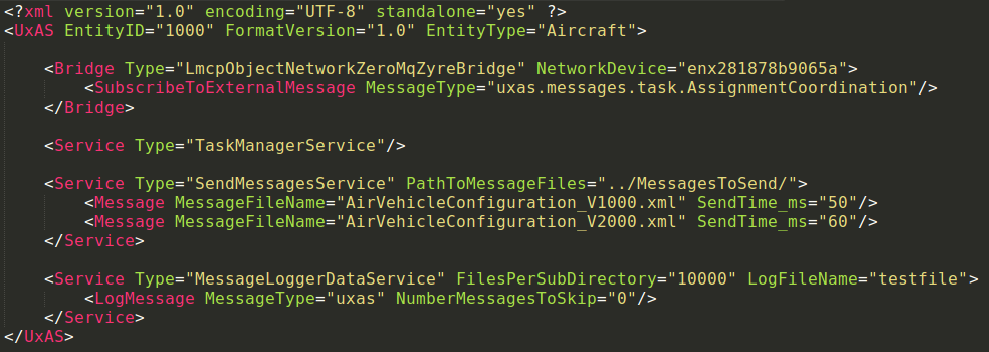
\includegraphics[width=1.3\linewidth]{\FiguresPath//ConfigExample}
	\caption{Sample configuration file}
	\label{fig:configExample}
\end{marginfigure}

Here is the \textbf{XML Declaration}:
\begin{docspec}<?xml version="1.0" encoding="UTF-8" standalone="yes" ?>\end{docspec}
The \textbf{UxAS Element}:
\begin{docspec}
	<UxAS EntityID="1000" FormatVersion="1.0" EntityType="Aircraft">
\end{docspec}
accepts the following attributes:
\begin{description}
	\item[\textit{EntityID}] Identification number of the entity represented by this instance of UxAS
	%\item[\textit{FormatVersion}] description ??????
	\item[\textit{EntityType}] used to differentiate between entities such as, \textit{Aircraft} and \textit{UGS}. Entries are defined by the services that use them.
	\item[\textit{ConsoleLoggerSeverityLevel}] if this attribute is present, all log messages at or below the severity level are displayed in the console. Valid entries are: \textit{DEBUG}, \textit{INFO}, \textit{WARN}, and \textit{ERROR}
	\item[\textit{MainFileLoggerSeverityLevel}] if this attribute is present, all log messages at or below the severity level are save in log files. Valid entries are: \textit{DEBUG}, \textit{INFO}, \textit{WARN}, and \textit{ERROR}
	%\item[\textit{StartDelay\_ms}] description
	\item[\textit{RunDuration\_s}] UxAS will run for \textit{RunDuration\_s} seconds before terminating.
	%\item[\textit{isLoggingThreadId}] description
\end{description}
Service Elements configure the services. There can be as many Service Elements as required. The attributes of the Service Elements are the options defined by each service. For example, the HelloWorld service can be configured with the following Service Element:
\begin{docspec}
	<Service Type="HelloWorld" StringToSend="Hello from \#1" SendPeriod\_ms="1000"/>
\end{docspec}
Bridge Elements configure bridges, which are services that create communication connections. For the Distributed Cooperation example, the zyre connection is configured with the following Bridge Element:
\begin{docspec}
    <Bridge Type="LmcpObjectNetworkZeroMqZyreBridge" NetworkDevice="enx281878b9065a">
	\quad<SubscribeToExternalMessage MessageType="uxas.messages.task.AssignmentCoordination"/>
	</Bridge>
\end{docspec}




\section{Core Services}
\begin{description}
	\item[\textbf{\textit{00\_ServiceTemplate}}] - This is a basic service that can be used as a template when constructing new services.
	\item[\textbf{\textit{01\_HelloWorld}}] - This is a basic example of a UxAS service that sends/receives KeyValuePair messages and prints out the results.
	\item[\textbf{\textit{AssignmentTreeBranchBoundService}}] - This service calculates assignments of vehicles to tasks based on cost inputs. 
	\item[\textbf{\textit{AutomationRequestValidatorService}}] - Checks all elements of automation requests to make sure they are present before sending out a UniqueAutomationRequest. 
	\item[\textbf{\textit{BatchSummaryService}}] - 
	\item[\textbf{\textit{MessageLoggerDataService}}] - This service logs messages received from other UxAS services to a SQLite database.  Logging can be configured to log either all or a subset of service messages.
	\item[\textbf{\textit{OperatingRegionStateService}}] - 
	\item[\textbf{\textit{OsmPlannerService}}] - loads an Open Street Map file and constructs ground plans/costs to be used for assignments.
	\item[\textbf{\textit{PlanBuilderService}}] - constructs plans from assignments. 
	\item[\textbf{\textit{RouteAggregatorService}}] - incrementally queries the route planner to build a matrix of plans between all tasks and entity initial points 
	\item[\textbf{\textit{RoutePlannerVisibilityService}}] - A component that constructs plans/costs to be used for assignments.
	\item[\textbf{\textit{SendMessagesService}}] - sends out messages, loaded from files, at a given time or periodically.
	\item[\textbf{\textit{SensorManagerService}}] - A service that constructs sensor footprints, calculates GSDs, determine sensor settings.
	\item[\textbf{\textit{ServiceBase}}] - the base class for all UxAS service classes. Service class constructors are registered in the \textit{ServiceBase} creation registry.
	\item[\textbf{\textit{ServiceManager}}] - a singleton class that inherits from the  \textit{ServiceBase}  class. It performs initial service creation for the UxAS entity at startup. After entity startup, it creates services per requests received from other services via messaging.  The ServiceManager  exclusively uses the  \textit{ServiceBase} creation registry to create services.
	\item[\textbf{\textit{WaypointPlanManagerService}}] -serves waypoint plans to the vehicle interface.
\end{description}

\section{Core Tasks}
\begin{description}
	\item[\textbf{\textit{00\_TaskTemplate}}] - This is a basic task that can be used as a template when constructing new tasks
	\item[\textbf{\textit{AngledAreaSearchTaskService}}] - Area search task with specified direction 
	\item[\textbf{\textit{BlockadeTaskService}}] - Task for using multiple vehicles to surround an entity, for example, multiple surface vehicles surrounding incoming enemy ship.
	\item[\textbf{\textit{CmasiAreaSearchTaskService}}] - Area search task
	\item[\textbf{\textit{CmasiLineSearchTaskService}}] - Defines a line search task. A line search is a list of points that forms a polyline. The ViewAngleList determines from which direction the line may be viewed. View angles are specified using the Wedge type. If the UseInertialViewAngles option is true, then wedges are defined in terms of North-East coordinates, otherwise wedges are defined relative to the line segment currently being viewed (a vector from point i through point i+1). To be a valid look angle, the line segment must be viewed from an angle within the bounds of the wedge. 
	\item[\textbf{\textit{CmasiPointSearchTaskService}}] - Point search task 
	\item[\textbf{\textit{CommRelayTaskService}}] - Task for providing comm relay support  
	\item[\textbf{\textit{CordonTaskService}}] - Task for using multiple ground vehicles to block access to an area. Given a point to secure and a standoff distance, task identifies number (K) routes that must be blocked to successfully deny access to the area. If there are not enough eligible vehicles, then this task will use the maximum number of eligible vehicles in a best effort strategy which attempts to maximize radial coverage. 
	\item[\textbf{\textit{EscortTaskService}}] - Task for targeting surveillance at an offset of a moving entity, for example to scout ahead of a convoy. 
	\item[\textbf{\textit{ImpactLineSearchTaskService}}] - Defines a line search task. A line search is a list of points that forms a polyline. The ViewAngleList determines from which direction the line may be viewed. View angles are specified using the Wedge type. If the UseInertialViewAngles option is true, then wedges are defined in terms of North-East coordinates, otherwise wedges are defined relative to the line segment currently being viewed (a vector from point i through point i+1). To be a valid look angle, the line segment must be viewed from an angle within the bounds of the wedge.
	\item[\textbf{\textit{ImpactPointSearchTaskService}}] - Impact Point Search Task 
	\item[\textbf{\textit{OverwatchTaskService}}] - Multi vehicle overwatch task 
	\item[\textbf{\textit{PatternSearchTaskService}}] - Search task with specified search pattern 
	\item[\textbf{\textit{TaskManagerService}}] - A service that constructs/destroys tasks.
	\item[\textbf{\textit{TaskServiceBase}}] - A base service that implements storage/functions common to all tasks.
	
\end{description}


\section{Connection Services}
\begin{description}
	\item[\textbf{\textit{LmcpObjectNetworkPublishPullBridge}}] -    
	\item[\textbf{\textit{LmcpObjectNetworkSerialBridge}}] - 
	\item[\textbf{\textit{LmcpObjectNetworkSubscribePushBridge}}] - connects an external entity to the internal message bus using \textit{ZMQ\_SUB} and \textit{ZMQ\_PUSH} sockets.
	\item[\textbf{\textit{LmcpObjectNetworkTcpBridge}}] - connects an external TCP/IP stream to the internal message bus.
	\item[\textbf{\textit{LmcpObjectNetworkZeroMqZyreBridge}}] - provides network discovery and communications. Dynamically discovers and bridges with zero-many Zyre-enabled systems. 
	\item[\textbf{\textit{ZeroMqZyreBridge}}] - provides network discovery and communications. Dynamically discovers and bridges with zero-many Zyre-enabled systems.
\end{description}

\section{Logging and Data Capture Services}
\begin{description}
	\item[\textbf{\textit{?????}}]    
\end{description}




